\section{Experimental Setup}\label{sec:methods}

\begin{figure}
    \centering
    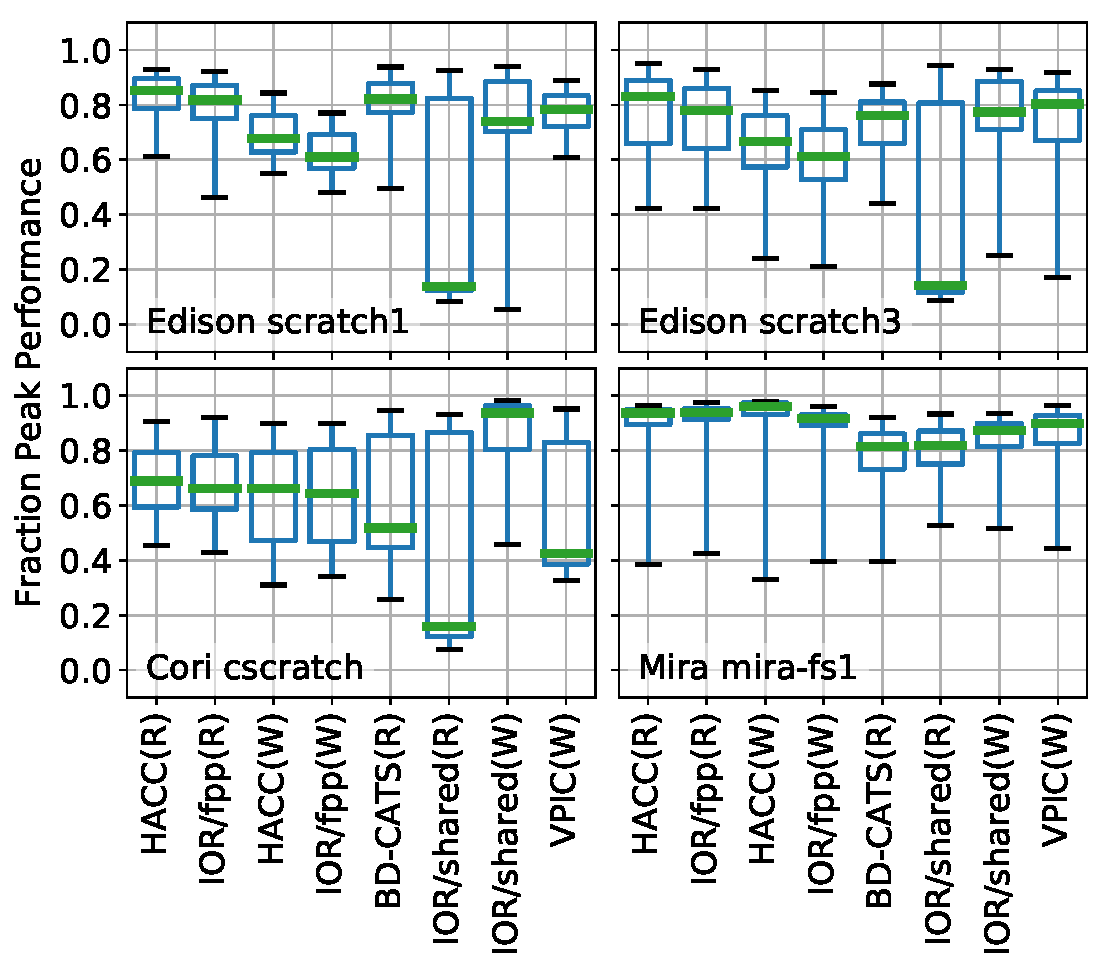
\includegraphics[width=0.9\columnwidth]{summary-boxplots}
    \vspace{-.15in}
    \caption{I/O performance grouped by test applications and read(R)/write(W) mode.  Whiskers represent the 5th and 95th percentiles.}
    \label{fig:summary-boxplots}
%   \vspace{-.3in}
\end{figure}

\begin{figure*}
    \centering
    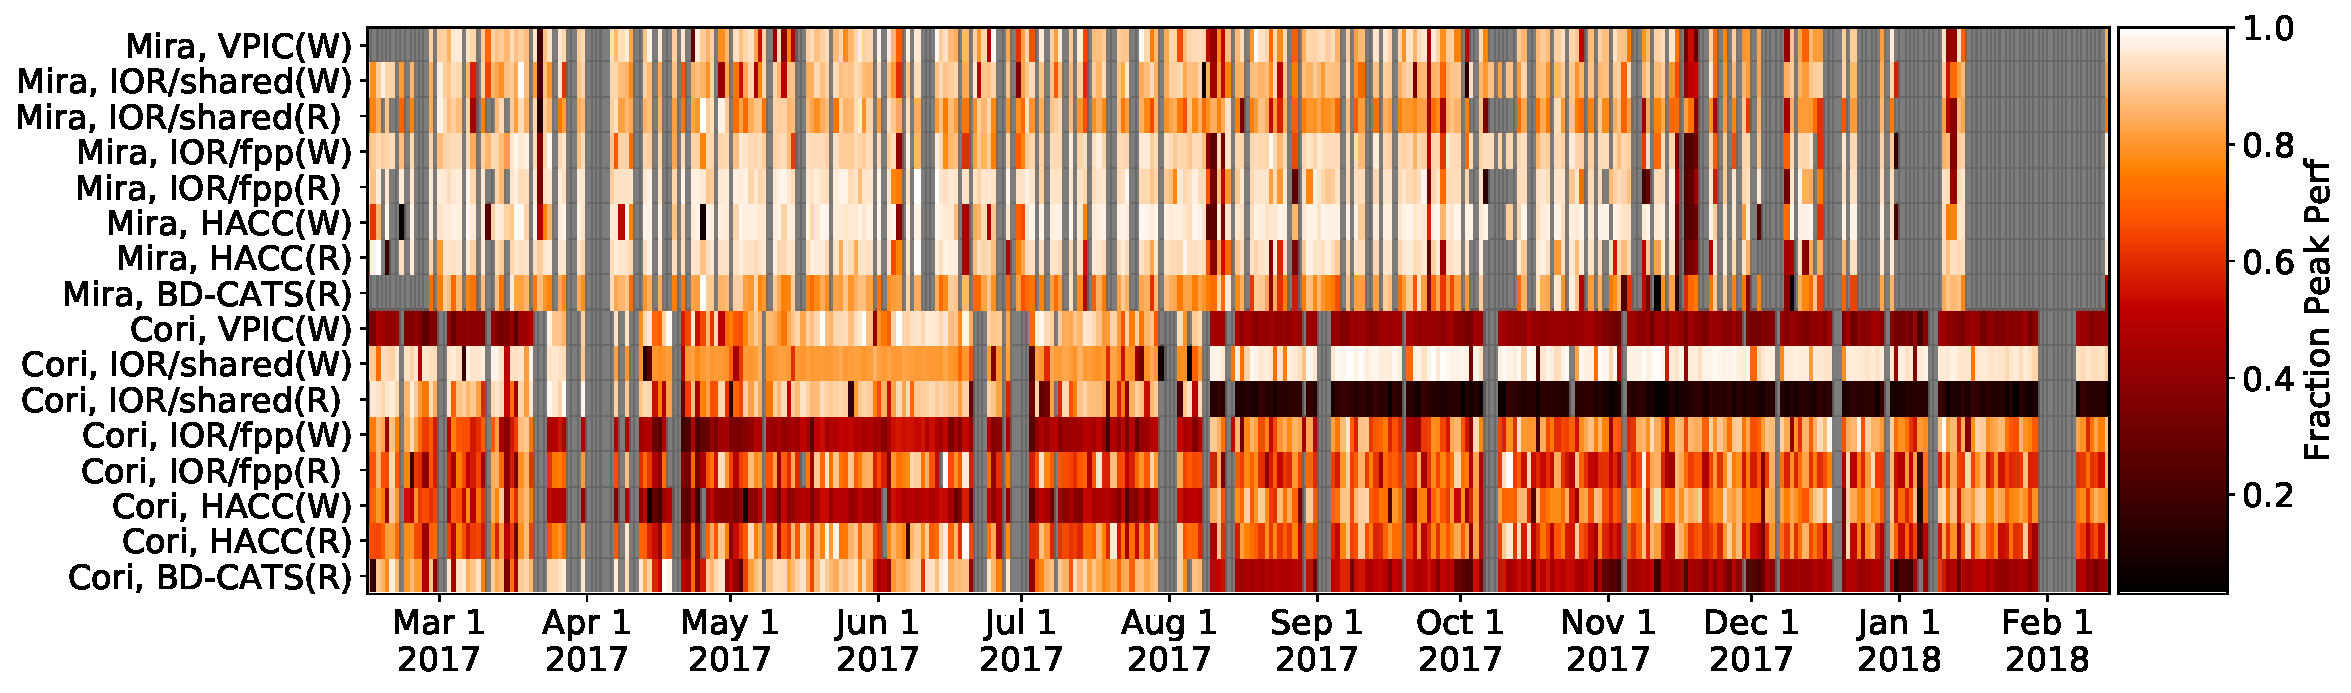
\includegraphics[width=0.90\linewidth]{summary-heatmap}
    \vspace{-.2in}
    \caption{Performance of daily benchmarks normalized to each benchmark's peak observed performance on the specified storage system.  The y-axis labels show combinations of system, I/O motif, and mode (Read/Write).  Grey represents days on which no observations were made.  The two regions highlighted in green boxes are expanded upon in Figure \ref{fig:regions-heatmap}.}
    \label{fig:summary-heatmap}
\end{figure*}

\TODO{How about changing this to ``Methodology'' section and have 'Data collection', 'Data characteristics', and 'Data analysis methods' as subsections, to make it sound this is the novel contribution of this effort? -- Suren}

\TODO{Need to accommodate double-blind review requirements while referring to \tokio.}

Previously, we have demonstrated the feasibility of a general approach to holistic I/O analysis of HPC systems and applied that approach over a month-long benchmarking study to examine specific cases of anomalous I/O behavior and to deduce potential factors contributing to this behavior~\cite{Lockwood2017}. We later formalized our methodology with the specification of the \tokio (\tokiolong) framework~\cite{Lockwood2018tokio}. For this work, we build on our prior research and use \tokio to analyze a massive amount of monitoring data culminating from a year-long I/O performance study conducted on a number of leadership-class HPC systems. 

In the following sections, we provide an overview of \tokio, describe the production HPC platforms we have deployed it on at NERSC and the ALCF, and describe our methodology for using a suite of daily I/O performance probes for active sampling of file system performance.

\subsection{\tokio Overview}\label{sec:methods/tokio}

%A holistic approach to understanding I/O behavior is a necessity given the move towards more complicated I/O architectures (in terms of number of constituent components, like high-level I/O libraries, I/O middleware systems, and low-level storage hardware) on these systems. \tokio's primary goal is to arm system users, administrators, and I/O researchers with the necessary tools to navigate this complexity and to make meaningful observations into how workloads interact with the I/O subsystem.

\tokio is a framework facilitating holistic characterization and analysis of I/O workloads running on today's production HPC systems. Conceptually, it provides an abstraction layer between component-level monitoring tools already deployed on HPC platforms and higher-level I/O analysis tools that utilize this data. The fundamental roles of the \tokio framework are to: collate monitoring data from distinct components; integrate and normalize the data from these components; and present coherent interfaces for indexing and accessing this data.
\TODO{Maybe a simple component diagram is useful if we have the space -SS}

\tokio boasts a modularized software architecture and a generic data format specification for system monitoring data, simplifying portability to new HPC platforms. Software modularity is accomplished by defining abstract \textit{connectors} to monitoring sources, each exposing interfaces for extracting relevant data in a format that is digestible by \tokio.  A generic timeseries format for monitoring data is also provided by \tokio, allowing for semantically consistent access to data originating from many distinct components (each with its own native format, scope, and granularity). This data format designates a number of metrics that are likely common to classes of monitoring components (e.g., file system monitoring tools likely gather common metrics, such as read/write bandwidths, operation counts, etc.). \tokio connectors can convert the native data formats of their underlying tools to this generic format in-memory as part of on-demand analysis, or \tokio-aware tools can archive directly into this format on-disk. These design decisions both greatly simplify the process of integrating new monitoring sources into the framework and the process of developing platform-independent I/O analysis tools.

Here, we briefly summarize monitoring sources supported by \tokio that are relevant to this particular study, though we refer readers to our previous work~\cite{Lockwood2017, Lockwood2018tokio} for a more comprehensive description of these sources (and other monitoring data sources supported by \tokio):

\begin{itemize}[leftmargin=*]
\item \textbf{Application-level monitoring}: \textit{Darshan}~\cite{Carns2009} is an application I/O characterization tool that is commonly deployed at production HPC facilities. It provides a condensed set of I/O counters, timers, and other statistics for each file accessed by a given application.

\item \textbf{File system workload monitoring}: \textit{LMT}~\cite{lmt} and \textit{ggiostat}~\cite{Lockwood2017} are examples of 
production-quality file system monitoring tools for Lustre and GPFS deployments, respectively. These tools each periodically capture metrics quantifying file system workloads over a given time interval, with some of these metrics being common to both tools (e.g., observed read/write bandwidths, number of specific I/O operations issued, etc.) and other metrics being file system specific (e.g., the CPU utilization on a given Lustre metadata server captured by LMT).

\item \textbf{File system capacity/health monitoring}: File system specific tools like Lustre's \textit{lfs} and \textit{lctl} or GPFS's \textit{mmdf} and \textit{mmlsdisk} can be invoked periodically to capture current file system state, including the capacity and failover status of individual storage servers and/or disks in the system.

\item \textbf{Job scheduler monitoring}: Job schedulers like Slurm~\cite{2003slurm} often keep a detailed accounting of all jobs that execute on a particular system, including useful details like the size of the job and its placement across available compute nodes.
\end{itemize}

\TODO{Worth giving the shoutout to the pytokio implementation here, or does that go in the reproducibility appendix?}

\subsection{HPC Platforms}\label{sec:methods/platforms}

% Please add the following required packages to your document preamble:
% \usepackage{multirow}
\begin{table}
\centering
\caption{Description of NERSC and ALCF test platforms.}
\label{tab:platform-descriptions}
\begin{tabular}{|c|c|c|c|c|}
\hline
                                                                                   & \textbf{Platform}                                                              & \textbf{FS Name (Type)} & \textbf{Size} & \textbf{Peak Rate}     \\ \hline
\multirow{3}{*}{\textbf{\begin{tabular}[c]{@{}c@{}}\edison\\ (\nersc)\end{tabular}}} & \multirow{3}{*}{\begin{tabular}[c]{@{}c@{}}Cray XC30\\ 5,586 CNs\end{tabular}} & scratch1                & 2.2 PiB       & 48 GB/sec              \\ \cline{3-5} 
                                                                                   &                                                                                & scratch2                & 2.2 PiB       & 48 GB/sec              \\ \cline{3-5} 
                                                                                   &                                                                                & scratch3                & 3.3 PiB       & 72 GB/sec              \\ \hline
\textbf{\begin{tabular}[c]{@{}c@{}}\cori\\ (\nersc)\end{tabular}}                    & \begin{tabular}[c]{@{}c@{}}Cray XC40\\ 12,076 CNs\end{tabular}                 & cscratch                & 28 PiB      & 744 GB/sec \\ \hline
\textbf{\begin{tabular}[c]{@{}c@{}}\mira\\ (\alcf)\end{tabular}}                     & \begin{tabular}[c]{@{}c@{}}IBM BG/Q\\ 49,152 CNs\end{tabular}                  & mira-fs1                & 7.0 PiB       & 90 GB/sec              \\ \hline
\end{tabular}
\end{table}

For this study, we deployed \tokio on the \edison and \cori systems at \nersc and the \mira system at the \alcf. Each of these platforms, along with their corresponding file systems analyzed as part of this study, are briefly described in Table~\ref{tab:platform-descriptions}.

Darshan is installed and automatically enabled on each of these systems, transparently characterizing the I/O workloads of a large portion of  each system's job population. 
\nersc has deployed LMT for full-time monitoring of the Lustre scratch volumes on both \edison and \cori, while the \alcf has deployed ggiostat to do the same with numerous GPFS volumes on \mira.
\nersc systems additionally utilize the Slurm job scheduler, which allows for the capture of detailed metadata for every job executed on \edison or \cori.
We additionally deployed \tokio on each of these systems, configuring it to leverage these existing monitoring sources in-place to provide a holistic view of I/O performance on each system.

\subsection{Active I/O Performance Probes}\label{sec:methods/benchmarks}

\begin{table}[b]
\centering
\caption{I/O Performance Probe Motifs}
\label{my-label}
\begin{tabular}{|r|c|c|}
\hline
\multicolumn{1}{|l|}{}    & \begin{tabular}[c]{@{}c@{}}$O(10^1 \textup{ MiB})$\\\textbf{Transfers}\end{tabular} & \begin{tabular}[c]{@{}c@{}}$O(10^2 \textup{ MiB})$\\\textbf{Transfers}\end{tabular} \\ \hline
\textbf{Shared File}      & IOR/shared                 & VPIC and BDCATS              \\ \hline
\textbf{File Per Process} & IOR/fpp                    & HACC                         \\ \hline
\end{tabular}
\label{tab:benchmark-motifs}
\end{table}

\begin{figure}
    \centering
    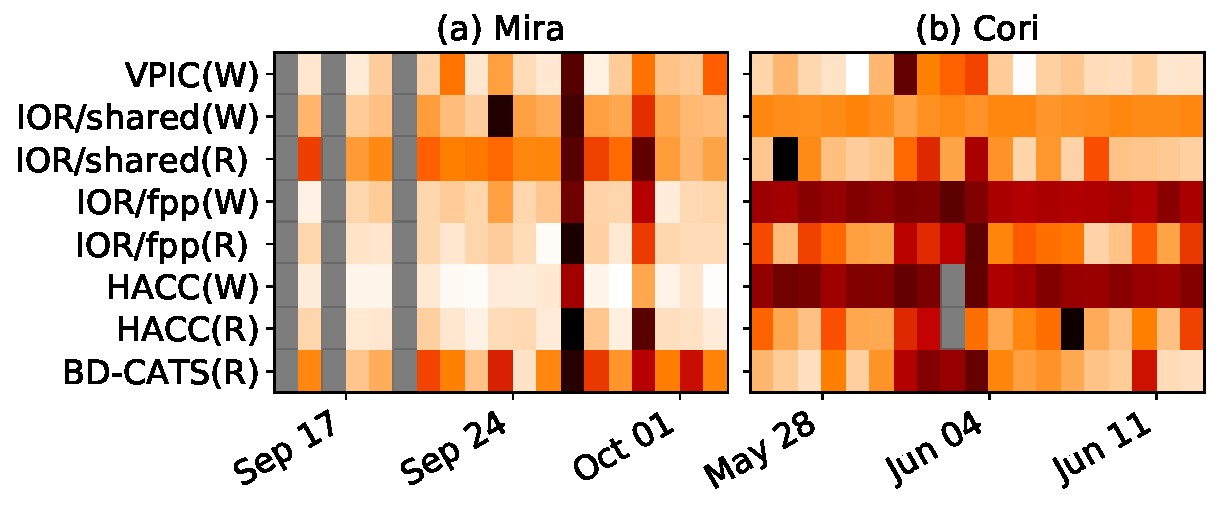
\includegraphics[width=0.90\linewidth]{regions-heatmap}
    \vspace{-.2in}
    \caption{Examples of structure in the fraction of peak performance observations.  Color scale is the same as that in Figure \ref{fig:summary-heatmap}.  In (a), the vertical band on Sept 26 corresponds to a transient system-wide degradation on \mira.  The horizontal bands for the IOR file-per-process write workload (IOR/fpp(W)) and HACC write workload (HACC(W)) in (b) show a sustained performance problem for file-per-process write workloads on \cori.}
    \label{fig:regions-heatmap}
\end{figure}

To measure the performance variation on the systems described in Section \ref{sec:methods/platforms}, we ran four I/O-intensive benchmarks on a daily basis from February 14, 2017 to February 15, 2018.
We utilize these benchmarking runs as another ad-hoc monitoring source for this study, actively probing the I/O performance of each analyzed file system on a daily basis across a range of representative I/O motifs.
The four underlying benchmarks (VPIC, BDCATS, HACC, and IOR) were configured to run identically to previous work~\cite{Lockwood2017} with the goal of using a substantial fraction of the I/O subsystem's peak bandwidth while using minimal production cycles.
These performance probes were chosen to exercise a variety of I/O workloads and covered the four I/O motifs listed in Table \ref{tab:benchmark-motifs} in both read and write modes.
The resulting 366-day experiment generated 11,986 performance observations across \mira, \cori, and \edison, reflecting 81.9\% of the intended probes having generated results.
The remaining 18.1\% of missing probes resulted from system downtime, malfunctions of component-level monitoring tools or the automated test scheduling, queue wait times that exceeded 24 hours, and benchmarks exceeding their walltime.
The fact that no results were obtained for jobs that ran so slowly that they exceeded their reserved walltime is significant in that this dataset does not capture the absolute worst performance observed.
Although not ideal, this reflects the realities of daily testing on production systems.
\TODO{Add details of the number of processes the benchmarks ran with, and how the file systems are set up, i.e., number of OSTs on \cori, number of I/O nodes used on \mira 
\\
\edison was mentioned in the previous paragraph; Figure 1 doesn't have the results. -- Suren}

% \TODO{Things that are important here: behavior over time, grouping data sources in a way that helps understand scope, focusing on fundamental \emph{changes} in performance rather than steady state, everything in one view.}

I/O performance is known to vary as a function of (1) the application I/O pattern, (2) whether the application is reading or writing, and (3) the architecture of the system on which I/O is happening~\cite{Lockwood2017}.
To remove the effects of these factors and enable us to focus on performance \emph{variation}, we therefore express the performance of each of the 11,986 observations $j$ in terms of its \emph{fraction of peak performance}.
This fraction of peak performance $j$ is defined as the absolute performance (in bytes/sec) of $j$ divided by the maximum absolute performance observed within the set $J_{app, rw, sys}$, where

\begin{equation}
J_{app, rw, sys} = \big\{ j_{app} \cap j_{rw} \cap j_{sys} \big \}
\end{equation}
\TODO{A little lost in Equation 1, may add more explanations on $j_{app}$, $j_{rw}$ and $j_{sys}$ -- Teng 
I don't think the set notation adds anything - Nick.}
\noindent
and $app$, $rw$, and $sys$ correspond to the three performance variables mentioned above.

An overview of the fraction of peak performance for two of the five systems tested is shown in Fig. \ref{fig:summary-boxplots} and demonstrates that the steady state for performance on production file systems is highly dynamic.
Further decomposition of two of these performance distributions is shown in Fig. \ref{fig:summary-heatmap} and reveals that performance variation is not randomly distributed over the year.
A significant amount of time-correlated structure, highlighted in Fig. \ref{fig:summary-heatmap}, demonstrates three phenomena commonly observed:

\begin{enumerate}[leftmargin=*]
\item Dark vertical bands, exemplified in the \mira data in Fig. \ref{fig:regions-heatmap}, represent transient system-wide issues that resulted in a uniform loss of performance for all applications tested that day.
\item Dark horizontal bands, shown in the \cori data, indicate a long-term degradation in performance that disproportionately affects a specific I/O motif or reads or writes.
\item Isolated dark blocks represent individual application runs where performance was poor despite an absence of system-wide transients (vertical bands) or systematic, motif-specific problems (horizontal bands).
\end{enumerate}

\TODO{Insert some smooth one-sentence transition into next section; perhaps mention that we don't consider the aforementioned results as surprising and the best is yet to come.}

The preponderance of these time-correlated phenomena underscore the need to consider variation as a function of time.
What may qualify as abnormally poor performance during one part of the year may be the baseline expected performance during another, and being able to understand these different regions of performance and variation is essential toward identifying and remedying their root causes.
It is therefore imperative to have a systematic approach towards identifying different regions of I/O performance to differentiate long-term performance degradation from shorter-term and transient variation.
In the following section, we describe a general approach to address this problem of partitioning performance measurements into regions of significant performance trends.

\TODO{In addition to above, maybe worth pointing out this is only showing results based on Darshan data, so we haven't even crossed into holistic territory, where datasets become much larger and difficult to analyze. -SS}

\TODO{Need to add definition of coverage factors somewhere}

